% Practice Test 19 — Indiana Edition
% Questions: 30 (23 MC + 7 SA)
% Generated by scripts/generate_practice_tests.py

\begin{practiceQuestion}{1-3-q01}{mc}
\begin{questionText}
What is the constant of proportionality ($k$) for the table below?

\begin{center}
\begin{tabular}{|c|c|}
\hline $x$ & $y$ \\ \hline $3$ & $12$ \\ $5$ & $20$ \\ $8$ & $32$ \\ \hline
\end{tabular}
\end{center}
\end{questionText}
\choiceA{$3$}
\choiceB{$4$}
\choiceC{$8$}
\choiceD{$12$}
\correctAnswer{B}
\explanation{$k = \frac{y}{x} = \frac{12}{3} = 4$. Check: $\frac{20}{5} = 4$ and $\frac{32}{8} = 4$.}
\end{practiceQuestion}

\begin{practiceQuestion}{1-5-q25}{sa}
\begin{questionText}
A proportional graph shows total cost versus hours of tutoring. The point $(3, 67.50)$ is on the graph. How much does $5$ hours of tutoring cost?
\end{questionText}
\correctAnswer{$\$112.50$}
\explanation{$k = \frac{67.50}{3} = 22.50$ per hour. Cost for $5$ hours: $22.50 \times 5 = \$112.50$.}
\end{practiceQuestion}

\begin{practiceQuestion}{1-6-q16}{mc}
\begin{questionText}
A factory produces $168$ items in $7$ hours. Another factory produces $200$ items in $8$ hours. Which factory is more productive?
\end{questionText}
\choiceA{Factory 1, at $24$ items/hr}
\choiceB{Factory 2, at $25$ items/hr}
\choiceC{They produce the same rate}
\choiceD{Factory 1, at $25$ items/hr}
\correctAnswer{B}
\explanation{Factory 1: $168 \div 7 = 24$ items/hr. Factory 2: $200 \div 8 = 25$ items/hr. Factory 2 is more productive.}
\end{practiceQuestion}

\begin{practiceQuestion}{2-2-q22}{sa}
\begin{questionText}
A school garden has $80$ plants. If $45\%$ are tomato plants, how many tomato plants are there?
\end{questionText}
\correctAnswer{$36$}
\explanation{$\frac{n}{80} = \frac{45}{100}$. Cross-multiply: $100n = 3600$. Divide: $n = 36$ tomato plants.}
\end{practiceQuestion}

\begin{practiceQuestion}{2-5-q01}{mc}
\begin{questionText}
A restaurant bill is $\$40$. You leave a $15\%$ tip. How much is the tip?
\end{questionText}
\choiceA{$\$4.00$}
\choiceB{$\$5.00$}
\choiceC{$\$6.00$}
\choiceD{$\$8.00$}
\correctAnswer{C}
\explanation{$15\% = 0.15$. Tip: $40 \times 0.15 = \$6.00$.}
\end{practiceQuestion}

\begin{practiceQuestion}{2-7-q03}{mc}
\begin{questionText}
In the percent error formula, why do we use absolute value?
\end{questionText}
\choiceA{To make the calculation easier}
\choiceB{Because the answer must be positive}
\choiceC{Because we only care about the size of the error, not the direction}
\choiceD{To convert the answer to a percent}
\correctAnswer{C}
\explanation{Absolute value ensures the percent error is positive whether the estimate was too high or too low.}
\end{practiceQuestion}

\begin{practiceQuestion}{3-1-q18}{mc}
\begin{questionText}
Which statement about absolute value is FALSE?
\end{questionText}
\choiceA{$|{-5}| = 5$}
\choiceB{$|0| = 0$}
\choiceC{Absolute value can be negative}
\choiceD{$|3| = |{-3}|$}
\correctAnswer{C}
\explanation{Absolute value measures distance from $0$, which is always $\geq 0$. It can never be negative.}
\end{practiceQuestion}

\begin{practiceQuestion}{3-2-q21}{sa}
\begin{questionText}
A hiker starts at an elevation of $-30$ feet (below sea level). She climbs $45$ feet. What is her new elevation?
\end{questionText}
\correctAnswer{$15$ feet}
\explanation{$(-30) + 45 = 15$. She is now $15$ feet above sea level.}
\end{practiceQuestion}

\begin{practiceQuestion}{4-2-q11}{mc}
\begin{questionText}
How many terms are in the simplified form of $8b - 3 + 2b + 5 - b$?
\end{questionText}
\choiceA{$5$}
\choiceB{$3$}
\choiceC{$2$}
\choiceD{$1$}
\correctAnswer{C}
\explanation{Combine variable terms: $8b + 2b - b = 9b$. Combine constants: $-3 + 5 = 2$. Simplified: $9b + 2$, which has $2$ terms.}
\end{practiceQuestion}

\begin{practiceQuestion}{4-3-q02}{mc}
\begin{questionText}
Expand $5(2a - 3)$.
\end{questionText}
\choiceA{$10a - 3$}
\choiceB{$7a - 3$}
\choiceC{$10a - 15$}
\choiceD{$10a + 15$}
\correctAnswer{C}
\explanation{$5 \times 2a = 10a$ and $5 \times (-3) = -15$. Result: $10a - 15$.}
\end{practiceQuestion}

\begin{practiceQuestion}{5-4-q12}{mc}
\begin{questionText}
Solve $\dfrac{n}{2} + \dfrac{n}{3} = 10$.
\end{questionText}
\choiceA{$n = 15$}
\choiceB{$n = 12$}
\choiceC{$n = 6$}
\choiceD{$n = 20$}
\correctAnswer{B}
\explanation{Multiply every term by $6$: $3n + 2n = 60$. Combine: $5n = 60$. Divide by $5$: $n = 12$. Check: $\frac{12}{2} + \frac{12}{3} = 6 + 4 = 10$ \checkmark.}
\end{practiceQuestion}

\begin{practiceQuestion}{5-5-q21}{sa}
\begin{questionText}
Write an inequality: ``A number $x$ divided by $4$, minus $3$, is at least $2$.'' Then solve.
\end{questionText}
\correctAnswer{$\dfrac{x}{4} - 3 \geq 2$; $x \geq 20$}
\explanation{$\frac{x}{4} - 3 \geq 2$. Add $3$: $\frac{x}{4} \geq 5$. Multiply by $4$: $x \geq 20$.}
\end{practiceQuestion}

\begin{practiceQuestion}{5-6-q27}{gmc}
\begin{questionText}
Which graph correctly shows the solution to $2x - 5 > 3$?

\textbf{Graph A:}
\begin{center}
\begin{tikzpicture}[scale=0.5]
  \draw[thick,->] (-1,0) -- (10,0);
  \foreach \x in {0,...,9} \draw (\x,0.12) -- (\x,-0.12) node[below,font=\small] {$\x$};
  \draw[thick,funBlue,->] (4,0) -- (10,0);
  \draw[thick,funBlue,fill=white] (4,0) circle (4pt);
\end{tikzpicture}
\end{center}

\textbf{Graph B:}
\begin{center}
\begin{tikzpicture}[scale=0.5]
  \draw[thick,->] (-1,0) -- (10,0);
  \foreach \x in {0,...,9} \draw (\x,0.12) -- (\x,-0.12) node[below,font=\small] {$\x$};
  \draw[thick,funOrange,->] (4,0) -- (10,0);
  \fill[funOrange] (4,0) circle (4pt);
\end{tikzpicture}
\end{center}

\textbf{Graph C:}
\begin{center}
\begin{tikzpicture}[scale=0.5]
  \draw[thick,->] (-1,0) -- (10,0);
  \foreach \x in {0,...,9} \draw (\x,0.12) -- (\x,-0.12) node[below,font=\small] {$\x$};
  \draw[thick,funGreen,<-] (-1,0) -- (4,0);
  \draw[thick,funGreen,fill=white] (4,0) circle (4pt);
\end{tikzpicture}
\end{center}
\end{questionText}
\choiceA{Graph A}
\choiceB{Graph B}
\choiceC{Graph C}
\choiceD{None of the above}
\correctAnswer{A}
\explanation{Solve: $2x > 8$, so $x > 4$. This is an open circle at $4$, shade right — Graph A.}
\end{practiceQuestion}

\begin{practiceQuestion}{6-1-q22}{sa}
\begin{questionText}
The actual length of a bridge is $360$ m. On a scale drawing, the bridge is $12$ cm. What is the scale in the form ``$1$ cm $= \underline{\quad}$ m''?
\end{questionText}
\correctAnswer{$1$ cm $= 30$ m}
\explanation{$360 \div 12 = 30$. The scale is $1$ cm $= 30$ m.}
\end{practiceQuestion}

\begin{practiceQuestion}{6-3-q06}{mc}
\begin{questionText}
You know all three angles of a triangle: $50°$, $60°$, and $70°$. How many triangles can be drawn?
\end{questionText}
\choiceA{None}
\choiceB{Exactly one}
\choiceC{Exactly three}
\choiceD{More than one (infinitely many)}
\correctAnswer{D}
\explanation{Three angles (AAA) determine the shape but not the size. You can draw infinitely many similar triangles of different sizes with these angles.}
\end{practiceQuestion}

\begin{practiceQuestion}{6-4-q28}{gmc}
\begin{questionText}
The diagram shows two triangles. Both have angles $30°$, $60°$, and $90°$, but different side lengths. What does this demonstrate?

\begin{center}
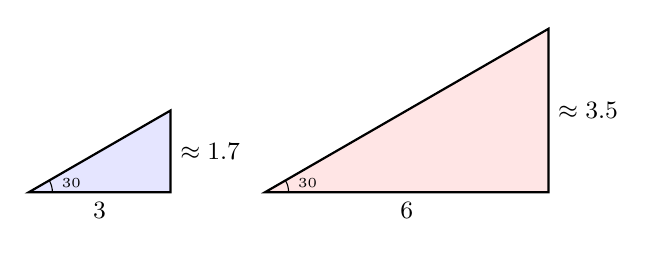
\begin{tikzpicture}[scale=0.6]
  % Small triangle
  \draw[thick,fill=blue!10] (0,0) -- (3,0) -- (3,1.73) -- cycle;
  \node[below] at (1.5,0) {\small $3$};
  \node[right] at (3,0.86) {\small $\approx 1.7$};
  \draw (0.5,0) arc[start angle=0,end angle=30,radius=0.5];
  \node at (0.9,0.2) {\tiny $30°$};
  % Large triangle
  \draw[thick,fill=red!10] (5,0) -- (11,0) -- (11,3.46) -- cycle;
  \node[below] at (8,0) {\small $6$};
  \node[right] at (11,1.73) {\small $\approx 3.5$};
  \draw (5.5,0) arc[start angle=0,end angle=30,radius=0.5];
  \node at (5.9,0.2) {\tiny $30°$};
\end{tikzpicture}
\end{center}
\end{questionText}
\choiceA{SSS produces multiple triangles}
\choiceB{AAA produces a unique triangle}
\choiceC{AAA produces multiple triangles of different sizes}
\choiceD{These two triangles are congruent}
\correctAnswer{C}
\explanation{Both triangles have the same angles but different side lengths. AAA determines shape but not size, so many triangles are possible.}
\end{practiceQuestion}

\begin{practiceQuestion}{6-5-q14}{mc}
\begin{questionText}
Which cross-section is NOT possible from slicing a rectangular prism?
\end{questionText}
\choiceA{Rectangle}
\choiceB{Triangle}
\choiceC{Circle}
\choiceD{Pentagon}
\correctAnswer{C}
\explanation{A rectangular prism has flat faces and straight edges. Its cross-sections can be triangles, rectangles, pentagons, or hexagons, but never circles (since it has no curved surfaces).}
\end{practiceQuestion}

\begin{practiceQuestion}{6-6-q13}{mc}
\begin{questionText}
Two lines intersect. One angle formed is $130°$. What are the measures of all four angles?
\end{questionText}
\choiceA{$130°$, $130°$, $50°$, $50°$}
\choiceB{$130°$, $50°$, $130°$, $100°$}
\choiceC{$130°$, $130°$, $130°$, $130°$}
\choiceD{$130°$, $60°$, $130°$, $40°$}
\correctAnswer{A}
\explanation{Vertical angles are equal ($130°$ and $130°$). Adjacent angles are supplementary: $180° - 130° = 50°$. The four angles are $130°$, $50°$, $130°$, $50°$.}
\end{practiceQuestion}

\begin{practiceQuestion}{6-7-q14}{mc}
\begin{questionText}
A rectangle has vertices $A(1, 1)$, $B(5, 1)$, $C(5, 3)$, $D(1, 3)$. It is translated left $3$ and up $4$. What are the coordinates of $C'$?
\end{questionText}
\choiceA{$(2, 7)$}
\choiceB{$(8, 7)$}
\choiceC{$(2, -1)$}
\choiceD{$(8, -1)$}
\correctAnswer{A}
\explanation{$C(5, 3)$: left $3$ means $5 - 3 = 2$, up $4$ means $3 + 4 = 7$. So $C'(2, 7)$.}
\end{practiceQuestion}

\begin{practiceQuestion}{7-3-q09}{mc}
\begin{questionText}
What is the area of a circle with a radius of $10$ cm? Use $\pi \approx 3.14$.
\end{questionText}
\choiceA{$31.4$ cm$^2$}
\choiceB{$62.8$ cm$^2$}
\choiceC{$100$ cm$^2$}
\choiceD{$314$ cm$^2$}
\correctAnswer{D}
\explanation{$A = \pi r^2 = 3.14 \times 100 = 314$ cm$^2$.}
\end{practiceQuestion}

\begin{practiceQuestion}{7-4-q04}{mc}
\begin{questionText}
A shape is made of a square with side $8$ cm and a semicircle with diameter $8$ cm attached to one side. What is the area? Use $\pi \approx 3.14$.
\end{questionText}
\choiceA{$64$ cm$^2$}
\choiceB{$89.12$ cm$^2$}
\choiceC{$114.24$ cm$^2$}
\choiceD{$139.12$ cm$^2$}
\correctAnswer{B}
\explanation{Square: $8^2 = 64$ cm$^2$. Semicircle: $\frac{1}{2} \times \pi r^2 = \frac{1}{2} \times 3.14 \times 16 = 25.12$ cm$^2$. Total: $64 + 25.12 = 89.12$ cm$^2$.}
\end{practiceQuestion}

\begin{practiceQuestion}{7-5-q09}{mc}
\begin{questionText}
A rectangular prism has dimensions $7$ m by $4$ m by $3$ m. What is the area of the largest face?
\end{questionText}
\choiceA{$12$ m$^2$}
\choiceB{$21$ m$^2$}
\choiceC{$28$ m$^2$}
\choiceD{$84$ m$^2$}
\correctAnswer{C}
\explanation{The three pairs of faces have areas $7 \times 4 = 28$, $7 \times 3 = 21$, and $4 \times 3 = 12$ m$^2$. The largest is $28$ m$^2$.}
\end{practiceQuestion}

\begin{practiceQuestion}{7-6-q27}{gmc}
\begin{questionText}
The figure shows unit cubes stacked into an L-shape. Each cube has a side length of $1$ cm. What is the total volume?

\begin{center}
\begin{tikzpicture}[scale=0.45]
  % Bottom row: 5 cubes
  \foreach \x in {0,1,2,3,4} {
    \draw[thick,funBlue,fill=funBlue!10] (\x,0) rectangle (\x+1,1);
  }
  % Second row on left: 3 cubes
  \foreach \x in {0,1,2} {
    \draw[thick,funBlue,fill=funBlue!15] (\x,1) rectangle (\x+1,2);
  }
  % Third row on left: 3 cubes
  \foreach \x in {0,1,2} {
    \draw[thick,funBlue,fill=funBlue!20] (\x,2) rectangle (\x+1,3);
  }
\end{tikzpicture}
\end{center}
\end{questionText}
\choiceA{$8$ cm$^3$}
\choiceB{$11$ cm$^3$}
\choiceC{$15$ cm$^3$}
\choiceD{$33$ cm$^3$}
\correctAnswer{B}
\explanation{Bottom row: $5$ cubes. Second row: $3$ cubes. Third row: $3$ cubes. Total: $5 + 3 + 3 = 11$ cm$^3$.}
\end{practiceQuestion}

\begin{practiceQuestion}{8-1-q22}{sa}
\begin{questionText}
Give one reason why a sample might not perfectly represent a population.
\end{questionText}
\correctAnswer{Random variation (or the sample may be biased)}
\explanation{Even a well-chosen random sample may differ slightly from the population due to chance.}
\end{practiceQuestion}

\begin{practiceQuestion}{8-3-q03}{mc}
\begin{questionText}
When comparing two populations visually, you should look at:
\end{questionText}
\choiceA{Only the center (mean or median)}
\choiceB{Only the spread (range or MAD)}
\choiceC{Both the center and the spread}
\choiceD{Only the largest and smallest values}
\correctAnswer{C}
\explanation{A complete comparison requires looking at both center (where the data clusters) and spread (how spread out it is).}
\end{practiceQuestion}

\begin{practiceQuestion}{8-4-q13}{mc}
\begin{questionText}
Store A daily sales: mean $\$500$, MAD $\$40$. Store B daily sales: mean $\$620$, MAD $\$40$. The difference in means in MADs is:
\end{questionText}
\choiceA{$1.5$ MADs}
\choiceB{$3$ MADs}
\choiceC{$40$ MADs}
\choiceD{$120$ MADs}
\correctAnswer{B}
\explanation{Difference $= \$620 - \$500 = \$120$. In MADs: $\frac{120}{40} = 3$ MADs.}
\end{practiceQuestion}

\begin{practiceQuestion}{8-7-q16}{mc}
\begin{questionText}
A line graph shows a plant's height each week: Week 1: $2$ cm, Week 2: $5$ cm, Week 3: $9$ cm, Week 4: $14$ cm. Between which weeks did the plant grow the most?
\end{questionText}
\choiceA{Week 1 to Week 2}
\choiceB{Week 2 to Week 3}
\choiceC{Week 3 to Week 4}
\choiceD{Growth was the same each week}
\correctAnswer{C}
\explanation{Week 1--2: $3$ cm. Week 2--3: $4$ cm. Week 3--4: $5$ cm. The most growth was Week 3 to 4.}
\end{practiceQuestion}

\begin{practiceQuestion}{9-4-q07}{mc}
\begin{questionText}
A coin is weighted so that heads comes up $60\%$ of the time. What is the probability of tails?
\end{questionText}
\choiceA{$0.60$}
\choiceB{$0.50$}
\choiceC{$0.40$}
\choiceD{$0.30$}
\correctAnswer{C}
\explanation{$P(\text{tails}) = 1 - 0.60 = 0.40$. Since heads and tails have different probabilities, this is a non-uniform model.}
\end{practiceQuestion}

\begin{practiceQuestion}{9-6-q30}{gsa}
\begin{questionText}
Look at the tree diagram for flipping three coins. What is the probability of getting exactly $2$ tails? Write your answer as a fraction in simplest form.

\begin{center}
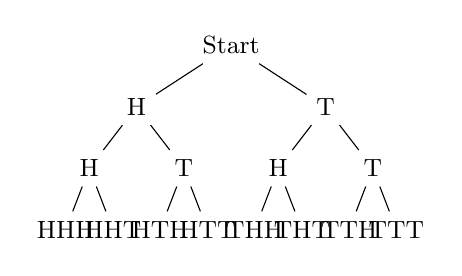
\begin{tikzpicture}[scale=0.6,
  level 1/.style={sibling distance=4cm, level distance=1.3cm},
  level 2/.style={sibling distance=2cm, level distance=1.3cm},
  level 3/.style={sibling distance=1cm, level distance=1.3cm}]
  \node {\small Start}
    child {node {\small H}
      child {node {\small H}
        child {node {\small HHH}}
        child {node {\small HHT}}
      }
      child {node {\small T}
        child {node {\small HTH}}
        child {node {\small HTT}}
      }
    }
    child {node {\small T}
      child {node {\small H}
        child {node {\small THH}}
        child {node {\small THT}}
      }
      child {node {\small T}
        child {node {\small TTH}}
        child {node {\small TTT}}
      }
    };
\end{tikzpicture}
\end{center}
\end{questionText}
\correctAnswer{$\frac{3}{8}$}
\explanation{Outcomes with exactly $2$ tails: HTT, THT, TTH — that is $3$ out of $8$. $P = \frac{3}{8}$.}
\end{practiceQuestion}

\begin{practiceQuestion}{9-7-q17}{mc}
\begin{questionText}
A student wants to simulate the probability that exactly $2$ out of $3$ students pass a test, where each student has a $50\%$ chance. Which model would work?
\end{questionText}
\choiceA{Roll one die: odd = pass, even = fail}
\choiceB{Flip $3$ coins: heads = pass, tails = fail; count exactly $2$ heads}
\choiceC{Draw $3$ marbles from a bag of $2$ red and $1$ blue}
\choiceD{Flip $1$ coin $3$ times and count all tails}
\correctAnswer{B}
\explanation{Each coin flip has a $50\%$ chance of heads (pass). Flipping $3$ coins and counting exactly $2$ heads simulates exactly $2$ passes.}
\end{practiceQuestion}
